\subsection{Verification and Analysis with UPPAAL}
\label{sec:mauppaal}
This section performs a formal analysis of the architectures of water tank. First of all, we encode FMUs of the water tank and model the MA with TA which composes a network of TA. Next, the models are verified with the model checker UPPAAL. The execution of FMU and co-simulation is time-related. We abstract the execution of FMUs for the water tank and encode it with the locations and transitions of TA according to the encoding rules proposed in Section \ref{sec:encoding}. Besides, we also model the MA as a TA to coordinate the execution between several FMUs. The TA templates for FMUs and MA are shown in Fig.\ref{tk-arch1}. Here, we adopt the rollback MA to coordinate the FMUs. The other two MAs can be analysed with the similar way. We do not present the details of them due to the space limits of this paper.

\begin{figure}[htbp]
\centering{
		\subfigure[TA for FMU\_controller]{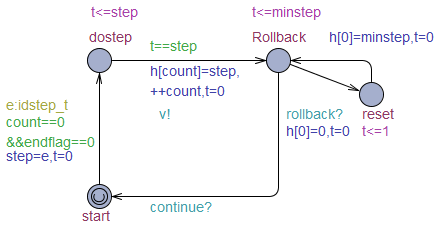
\includegraphics[width=1.6in,height=1.0in]{fig/2signal_controller.png}
			\label{tk_controller}}
		\hfil
		\subfigure[TA for FMU\_valve]{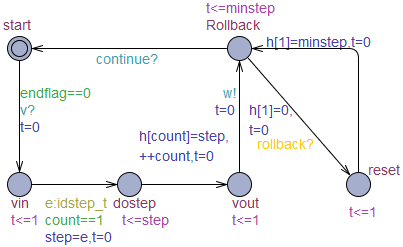
\includegraphics[width=1.6in,height=1.0in]{fig/2signal_v.png}
			\label{tk_v}}
			
	    \subfigure[TA for FMU\_WaterTank1]{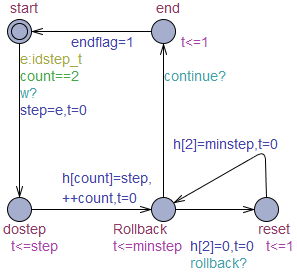
\includegraphics[width=1.5in,height=1.2in]{fig/2signal_wt1.png}
			\label{tk_wt1}}
		\hfil
		 \subfigure[TA for rollback MA]{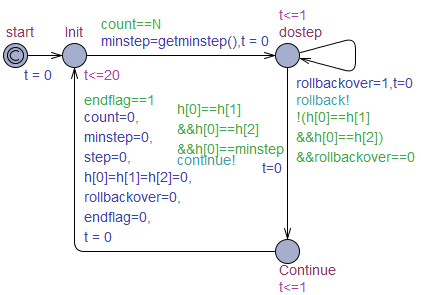
\includegraphics[width=1.7in,height=1.2in]{fig/2signal_master.png}
			\label{tk_ma}}		
	\caption{TA Network for connection case 1: $controller$ $\vert\vert$ $valve$ $\vert\vert$ $WaterTank1$ $\vert\vert$ $MA$.}
	\label{tk-arch1}
	}
\end{figure}

\begin{figure}[htbp]
\centering{
		\subfigure[Execution trace]{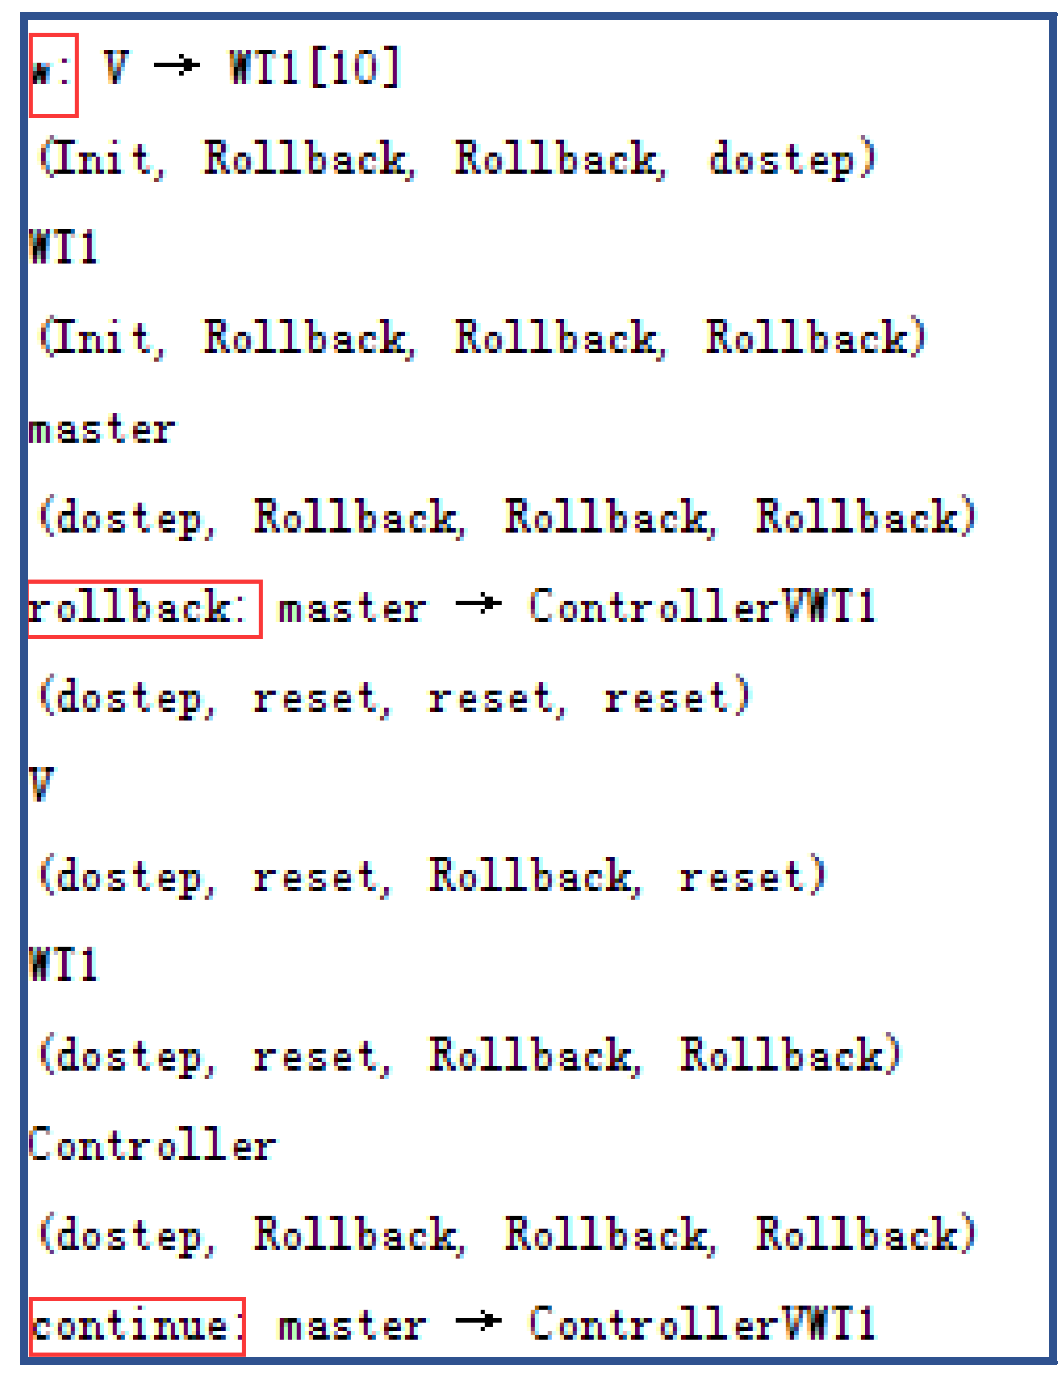
\includegraphics[width=1.6in,height=2.0in]{fig/trs.png}
			\label{trs}}
		\hfil
		\subfigure[Execution sequence diagram]{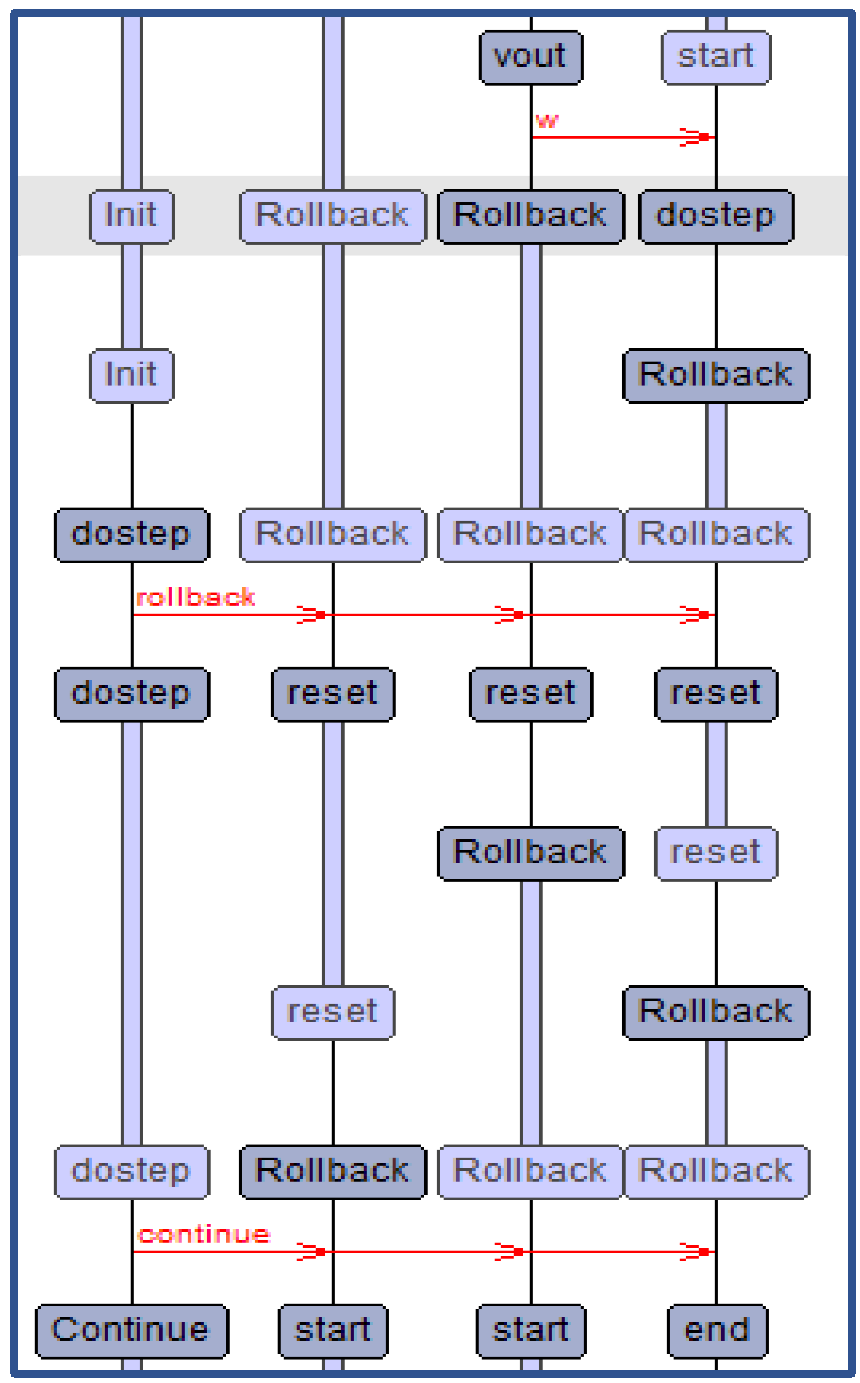
\includegraphics[width=1.6in,height=2.0in]{fig/seq.png}
			\label{seq}}
	\caption{The execution fragment of the coordination in UPPAAL.}
	\label{trs-seq}
	}
\end{figure}

Fig.~\ref{tk_controller}, \ref{tk_v}, \ref{tk_wt1} are the templates for $controller$, $valve$ and $WaterTank1$ respectively, which model FMUs of the water tank. These FMUs have four key states: $start$, $dostep$, $Rollback$ and $reset$. Fig.~\ref{tk_controller} shows the template for $controller$ which executes with the random step size. It synchronizes with $valve$ by signal $v$ and transfers to $Rollback$ state, and then waits for a signal from the MA. Until the $controller$ receives the $continue$ signal, it does data exchange with other FMUs, and returns to $start$ state. Otherwise, it receives $rollback$ signal, when it obtains the minimize step size of all FMUs, it transfers to $Rollback$ state. The states and transitions of $valve$ and $WaterTank1$ template are similar with the template of $controller$. Fig.~\ref{tk_ma} shows the template for the MA. Firstly, the MA initializes the parameters, and then it gets minimize step size of FMUs until all FMUs visit $dostep$. Next, the MA decides which signal should be sent according to the guard. If the step sizes of all FMUs are equal, the MA will send $continue$ signal, otherwise, send $rollback$ signal.

Fig.~\ref{trs-seq} is the execution fragment of the coordination in UPPAAL, we can find that $valve$ sends a $w$ signal to perform data exchange with $WaterTank1$. After that, $WaterTank1$ moves to $dostep$ state. The MA broadcasts a $rollback$ signal to all templates, which leads to all of them arrive at $reset$ state. Finally, the MA sends a $continue$ signal to all FMUs. All templates return to $start$ state, and then do the next step. The execution fragments show that our models are correct.

In order to compare the behavior of three connection cases of water tank system, we also model the other two connection cases in UPPAAL. For connection case 2, we add channel $s$ in the templates for $controller$ and $WaterTank1$ as shown in Fig.\ref{tk-arch2}. For connection case 3, we create template for $WaterTank2$ and channel $w2$ as shown in Fig.\ref{arc3}. The other models are the same as models of connection case1. Limited to the length of this paper, we only show the templates for $controller$ and $WaterTank1$ of connection case 2 and template for $WaterTank2$ of connection case 3. In the next subsection, we verify some properties of various connection cases to detect whether there is an algebraic loop in the architecture.
\begin{figure}[htbp]
\centering{
		\subfigure[TA for FMU\_controller]{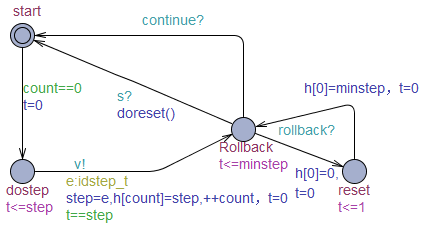
\includegraphics[width=1.8in,height=1.2in]{fig/2signal_cycle_controller.png}
			\label{tk2_controller}}
		\hfil
		\subfigure[TA for FMU\_WaterTank1]{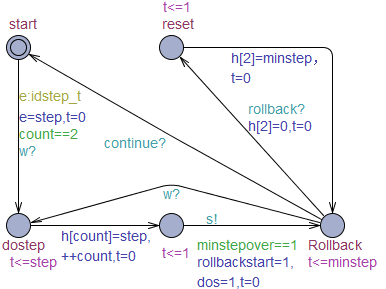
\includegraphics[width=1.5in,height=1.2in]{fig/2signal_cycle_wt1.png}
			\label{tk2_v}}		
	\caption{TA for connection case 2.}
	\label{tk-arch2}
	}
\end{figure}
\begin{figure}[htbp]
	\centering	{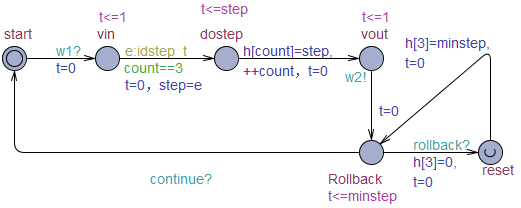
\includegraphics[width=3.5in,height=1.2in]{fig/4signal_wt2.png}}
	\caption{TA for FMU\_WaterTank2 of connection case 3.}\label{arc3}
\end{figure}

UPPAAL supports a simplified version of TCTL \cite{BouchenebGR09} to specify the property. We verify the following properties of each connection case:
\begin{itemize}
\item
$E\langle\rangle~WT1.Rollback$ and $E\langle\rangle~master.Continue$ specify reachability properties. It means the FMU of $WaterTank1$ will $Rollback$ and the MA will reach $Continue$ state.
\item
$master.start \rightarrow master.Continue$ specifies liveness property. It means once the MA start, it will continue eventually.
\item 
$A[]~not~deadlock$ specifies safety property. It means the execution of the system will not be deadlock.
\end{itemize}

The verification results are listed in Table \ref{rs}. We can find that all properties of connection case 1 and case 3 are satisfied. It shows that our MA works well and the composition of FMUs is determinate. However, the liveness and reachability properties of connection case 2 are not satisfied. It means there is an algebraic loop which may be introduced with the I/O dependency in the architecture. The experimental results show that our approach is feasible and useful for model checking the coordination of CPS. Here, we only focus on the detection of algebraic loop and the correctness of coordination. In the future work, we will consider how to eliminate the algebraic loop.  
\begin{table}
\caption{Experimental results for various connection case}
\centering
\begin{tabular}{c c c} 
        \hline  
        Connection case & Verified Property & Result\\
        \hline
        \multirow{2}{2.0cm}{Case 1}  
                & $E\langle\rangle~WT1.Rollback$ & True\\ 
                & $E\langle\rangle~master.Continue$ & True\\ 
                & $master.start\rightarrow master.Continue$ & True\\ 
                & $A[]~not~deadlock$ & True\\   
        \hline 
        \multirow{2}{2.0cm}{Case 2}  
                & $E\langle\rangle~WT1.Rollback$ & True\\ 
                & $E\langle\rangle~master.Continue$ & False\\ 
                & $master.start\rightarrow master.Continue$ & False\\ 
                & $A[]~not~deadlock$ & True\\   
        \hline 
        \multirow{2}{2.0cm}{Case 3}  
                & $E\langle\rangle~WT1.Rollback$ & True\\ 
                & $E\langle\rangle~master.Continue$ & True\\ 
                & $master.start \rightarrow master.Continue$ & True\\ 
                & $A[]~not~deadlock$ & True\\   
        \hline 
\end{tabular} 
\label{rs}
\end{table}




